\section{PATCH Patch Graphics Function}

\subsection{Usage}

This routine is used to create a patch object that can be plotting 2D and 3D surfaces.  A 
patch is a polygon defined by the xyz coordinates
of its vertices and optionally by the color at the vertices.
There are several forms for the \verb|patch| function:
\begin{verbatim}
  h = patch(X,Y,C,properties...)
  h = patch(X,Y,Z,C,properties...)
  h = patch(properties...)
  h = patch(V)
\end{verbatim}
Where \verb|X|, \verb|Y| and \verb|Z| are matrices or vectors of \verb|x|, \verb|y| or \verb|z| coordinates
and \verb|C| is a matrix or vector of color values (the colormap
for the current fig is applied).  
\subsection{Example}

Here we generate a surface specifying all four components.
\begin{verbatim}
--> x = [ 0 1 0 1]';
--> y = [ 0 0 1 1]';
--> c = [ 1 1 1 ];
--> patch(x,y,c)
--> axis equal
--> view(3)
\end{verbatim}


\centerline{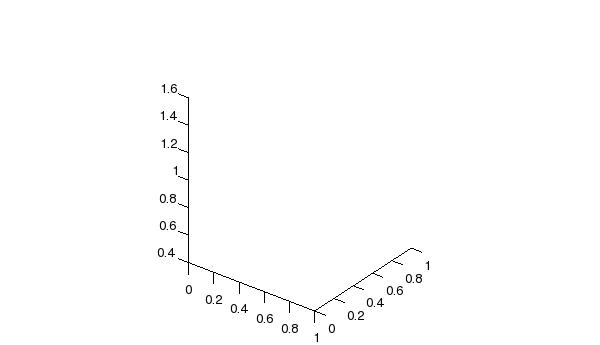
\includegraphics[width=8cm]{patch1}}

